\documentclass[../1.tex]{subfiles}
\begin{document}
    
    \label{section:1.1}

    In this section we shall define structures called simplicial complexes and discuss some of their properties. In order to define these structures
    we need the definitions of convex hull and affine independence in $\R^n$. In this chapter we recall some notions of algebraic topology, such as simplicial
    complexes and homology. For more details we invite the reader to consult \cite{hatcher}, a good reference also for the preliminary necessary notions of
    topology we are unable to treat here.    

    \begin{defn}
        Let $A \subset \R^n$, we define $A$ to be \ii{convex} if
        \[ x,y \in A \then tx + (1+t)y \in A \]
        for all $t \in [0,1]$.
    \end{defn}

    In \autoref{fig:1} can see in blue an example of a convex set: every segment joining two points of the set lies within the set.
    The green set is not convex, in fact we see that the segment in the illustration partially lies outside of the set.

    \begin{figure}[H]
        \centering
        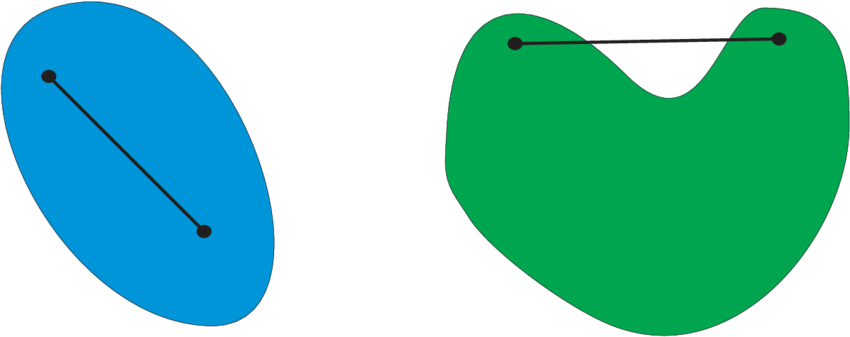
\includegraphics[width=8cm, height=4cm]{sections/1/convex}
        \caption{Illustration of a convex (blue) and a non-convex (green) set.}
        \label{fig:1}
    \end{figure}

    \begin{defn}
        Let $\sigma := \{x_i\}_{i \in I}$ be a subset of $\R^n$, where $I$ is a finite set of indexes, we define $\sigma$ to be \ii{affinely independent} if 
        $\{ x_0 - x_i\}_{i \in I \m \{0\}}$ is linearly independent.
    \end{defn}

    We show now that the definition of affine independence of $\sigma = \{x_i\}_{i \in I} \subset \R^n$ is independent of the choice of $x_0$.
      
    \begin{prop}
        Let $\sigma := \{x_i\}_{i \in I}$ be a finite subset of $\R^n$, let $j \in I$ then, if $\{ x_j - x_i\}_{i \in I \m \{j\}}$ is linearly independent,
        also $\{ x_0 - x_i\}_{i \in I \m \{0\}}$ is. 
    \end{prop}
    \begin{proof}
        If $j=0$ the statement is trivially true. Let $j \neq 0$ and $\lambda_i \in \R$ for all $i \neq j$, then
        \[ \sum_{i \in I \m \{j\}} \lambda_i (x_j - x_i) = 0 \then \lambda_i = 0 \quad \forall i \in I \m \{j\}.\]
        Let then $\mu_i \in \R$ for all $i \neq 0$, and suppose 
        \[ \sum_{i \in I \m \{0\}} \mu_i (x_0 - x_i) = (x_0 - x_j) \sum_{i \in I \m \{0\}} \mu_i + \sum_{i \in I \m \{0\}} \mu_i (x_j - x_i) = 0.\]
        If we define $\mu_0 := -\sum_{i \in I \m \{0\}} \mu_i$ we have that
        \[ 0 = \sum_{i \in I} \mu_i (x_j - x_i) = \sum_{i \in I \m \{j\}} \mu_i (x_j - x_i) \then \mu_i = 0 \quad \forall i \in I \m \{j\},\]
        which proves our proposition. the definition of affine ind the definition of affine independence is well stated. \qedhere
    \end{proof}

    \begin{defn}
        Let $\sigma := \{x_i\}_{i \in I}$ be a finite subset of $\R^n$, we define the \ii{convex set generated by $\sigma$} to be 
        the smallest convex set containing $X$ according to the inclusion relation. We shall denote this set by $[\sigma]$ and call 
        it \ii{convex hull} of $\sigma$.
    \end{defn}

    Since the intersection of convex sets is convex, the convex set generated by $\sigma$ can be equivalently defined as the intersection 
    of all convex sets containing $\sigma$.

    \begin{thm}
        Let $\sigma := \{x_i\}_{i \in I}$ be a finite subset of $\R^n$, if $\sigma$ is affinely independent then the convex set generated by $\sigma$ is 
        \[ [\sigma] = \{ \sum_{i \in I} \lambda_i x_i : \lambda_i \geq 0, \sum_{i \in I} \lambda_i = 1\}. \]
        Furthermore for any point $x \in [\sigma]$ we have that
        \[ x = \sum_{i \in I} \lambda_i x_i = \sum_{i \in I} \mu_i x_i \then \lambda_i = \mu_i \forall i \in I, \] 
        where $\lambda_i,\mu_i \geq 0$ and $\sum_{i \in I} \lambda_i = \sum_{i \in I} \mu_i =1$.
        \label{thm:1}
    \end{thm}

    \begin{proof}
        Let $C := \{ \bigcap_\alpha C_\alpha : \sigma \subset C_\alpha, C_\alpha$ convex$\}$, we divide the proof in three steps:
        \begin{enumerate}[(i)]
            \item $C \subset [\sigma]$.\\
            This is true if $[\sigma]$ is convex and contains $\sigma$.
            The proof that it contains $\sigma$ is trivial. In fact for every vertex $x_j = \sum_{i \in I} \delta_{ij} x_i$,
            and $\sum_{i \in I}\delta_{ij} = 1$.\\
            To prove that it is convex we chose two points $a = \sum_{i \in I} a_i x_i, b = \sum_{i \in I} b_i x_i$ \\
            where $a_i,b_i \geq 0 \; \forall i \in I$ and $\sum_{i \in I} a_i = \sum_{i \in I} b_i = 1$. For $t \in [0,1]$
            \[ ta+(1-t)b = t\sum_{i \in I} a_i x_i + (1-t) \sum_{i \in I} b_i x_i = \sum_{i \in I} (ta_i + (1-t)b_i)x_i.\]
            Since $ta_i + (1-t)b_i \geq 0$ and $\sum_{i \in I} (ta_i + (1-t)b_i) = t\sum_{i \in I}a_i + (1-t)\sum_{i \in I}b_i = 1$ for all $i \in I$,
            our statement is proven.

            \item $[\sigma] \subset C$.\\
            If all but one the $\lambda_i$ are zero certaintly $\sum_{i \in I} \lambda_i x_i \in C$, since $C$ contains all the vertexes.
            The inuctive hypothesis, by relabeling, is that if the first $\lambda_0,...,\lambda_{n-1}$ are non-zero, hence not even $1$, then $\sum_{i \in I} \lambda_i x_i \in C$.
            We want to show that whenever $\lambda_0,...,\lambda_n$ are non-zero then also $\sum_{i \in I} \lambda_i x_i \in C$, since $\lambda_n \neq 1$ we have that
            \[ \sum_{i \in I} \lambda_i x_i =  \sum_{i = 0}^n \lambda_i x_i = \lambda_n x_n + \sum_{i = 0}^{n-1} \lambda_i x_i =
               \lambda_n x_n + (1 - \lambda_n) \sum_{i = 0}^{n-1} \frac{\lambda_i}{1 - \lambda_n} x_i.\]
            Since $\sum_{i = 0}^{n-1} \frac{\lambda_i}{1 - \lambda_n} = 1$, for the inductive hypothesis $\sum_{i = 0}^{n-1} \frac{\lambda_i}{1 - \lambda_n} x_i \in C$.
            Also the vertex $x_n$ is contained in $C$ by definition, therefore, being $C$ convex and $\lambda_n \in [0,1]$, it follows that 
            \[ \lambda_n x_n + (1 - \lambda_n) \sum_{i = 0}^{n-1} \frac{\lambda_i}{1 - \lambda_n} x_i \in C. \]
            Accordingly $\sum_{i \in I} \lambda_i x_i \in C$, by induction we conclude the proof.

            \item $\sum_{i \in I} \lambda_i x_i = \sum_{i \in I} \mu_i x_i \then \lambda_i = \mu_i \forall i \in I$.\\
            Let $\sum_{i \in I} \lambda_i x_i = \sum_{i \in I} \mu_i x_i$, then also $x_0\sum_{i \in I} \lambda_i + \sum_{i \in I} \lambda_i(x_i-x_0) = 
            x_0\sum_{i \in I} \mu_i +\sum_{i \in I} \mu_i (x_i - x_0)$, and since both $\lambda_i$ and $\mu_i$ are normalised we have that
            \[ \sum_{i \in I} (\lambda_i - \mu_i) (x_0 - x_i) = \sum_{i \in I \m \{0\}} (\lambda_i - \mu_i) (x_0 - x_i) = 0 \then \lambda_i = \mu_i \quad \forall i \in I \m \{0\},\]
            because of the affine independence. \qedhere
        \end{enumerate}
    \end{proof}
  
    \begin{defn}
        We define a \ii{p-simplex} $[\sigma]$ to be the convex hull of an affinely independent set $\sigma := \{x_i\}_{i \in I} \subset \R^n$,
        where $p = |I|-1$ is called dimension of the $p$-simplex. 
    \end{defn}

    Theorem \ref{thm:1} gives us the possibility to represent a point in a simplex $[\sigma]$ via a finite set of real parameters defined in the range $[0,1]$
    and satisfying the normalisation condition $\sum_{i \in I } \lambda_i = 1$. Such parameters are called \ii{baricentric coordinates} of $[\sigma]$.\\
    \hfill \\
    The points in $\sigma$ are called \ii{vertexes} of the simplex $[\sigma]$, accordingly we define the vertex set of a simplex $[\sigma]$ to be 
    $Vert([\sigma]) = \sigma$.
    
    \begin{defn}
        Let $[\sigma]$ be a $p$-simplex and $p,t \in \N$, we say that another $t$-simplex $[\tau]$ is a \ii{face} of $[\sigma]$ or equivalently 
        that $[\sigma]$ is a \ii{coface} of $[\tau]$, and we write $[\tau] \leq [\sigma$], if $\tau \subset \sigma$, where $t \leq p$.
    \end{defn}

    Now we are ready for our main definitions.
    
    \begin{defn}
        We define a \ii{simplicial complex} $\mc{G}$ to be a collection of simplexes such that
        \begin{enumerate}[(i)]
            \item if any simplex $ [\tau] \leq [\sigma]$ and $[\sigma] \in \mc{G}$, then $ [\tau] \in \mc{G}$,
            \item if $ [\sigma], [\tau] \in \mc{G}$, then $[\sigma] \cap [\tau] \in \mc{G}$.
        \end{enumerate}
    \end{defn}

    \autoref{fig:2} represents a simplicial complex, while \autoref{fig:3} represents a collection of simplexes which is not a simplicial complex. 

    
    \begin{figure}[H]
        \centering
        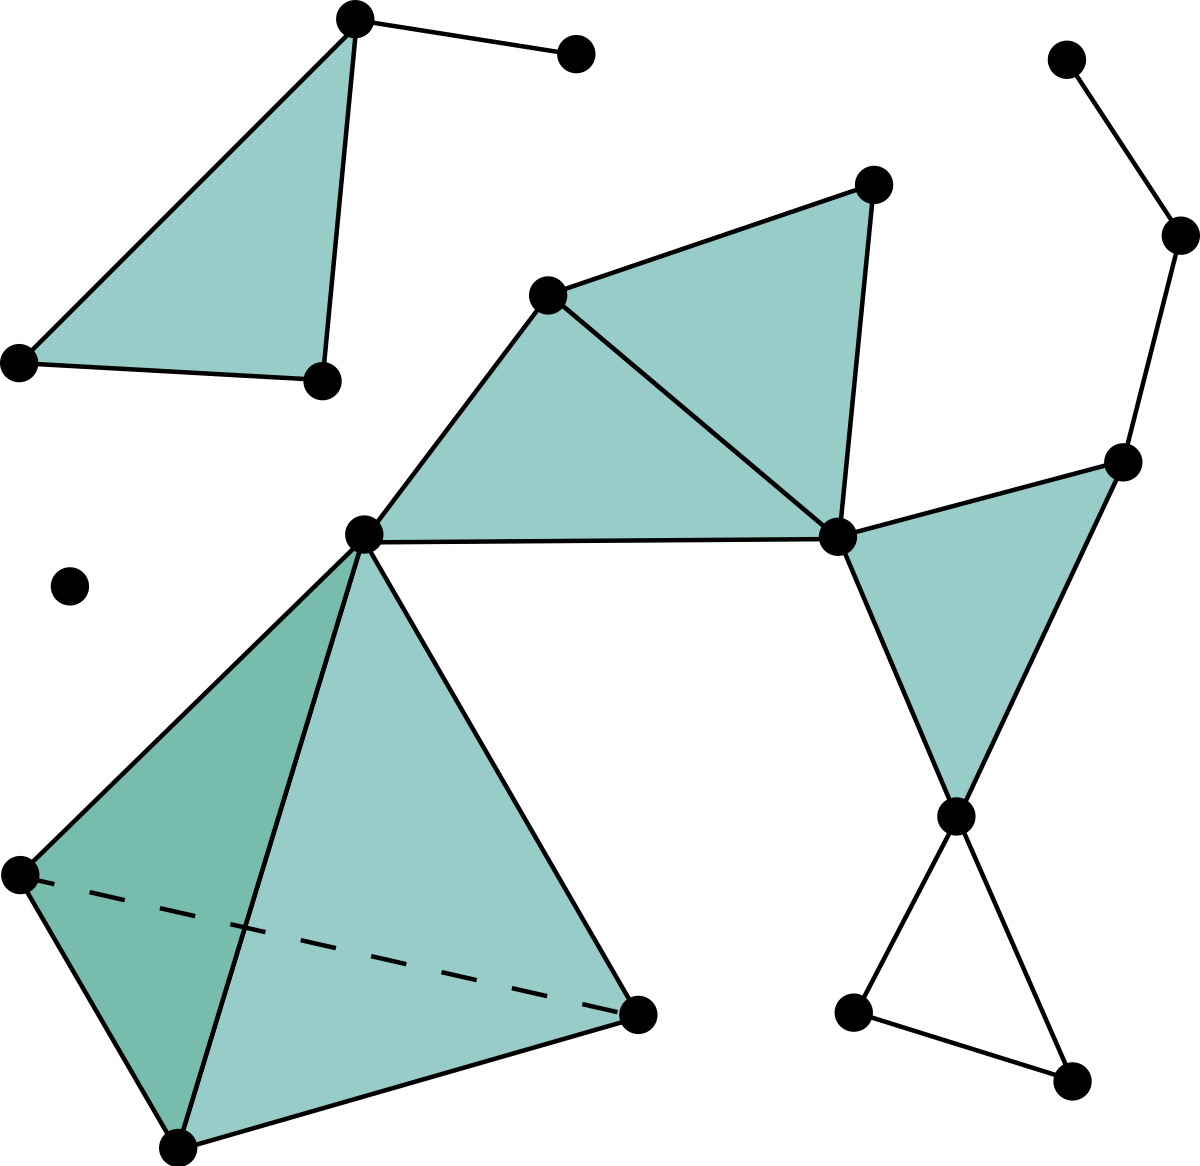
\includegraphics[width=4cm, height=4cm]{sections/1/complex}
        \caption{Example of simplicial complex.}
        \label{fig:2}
    \end{figure} 

    \begin{figure}[H]
        \centering
        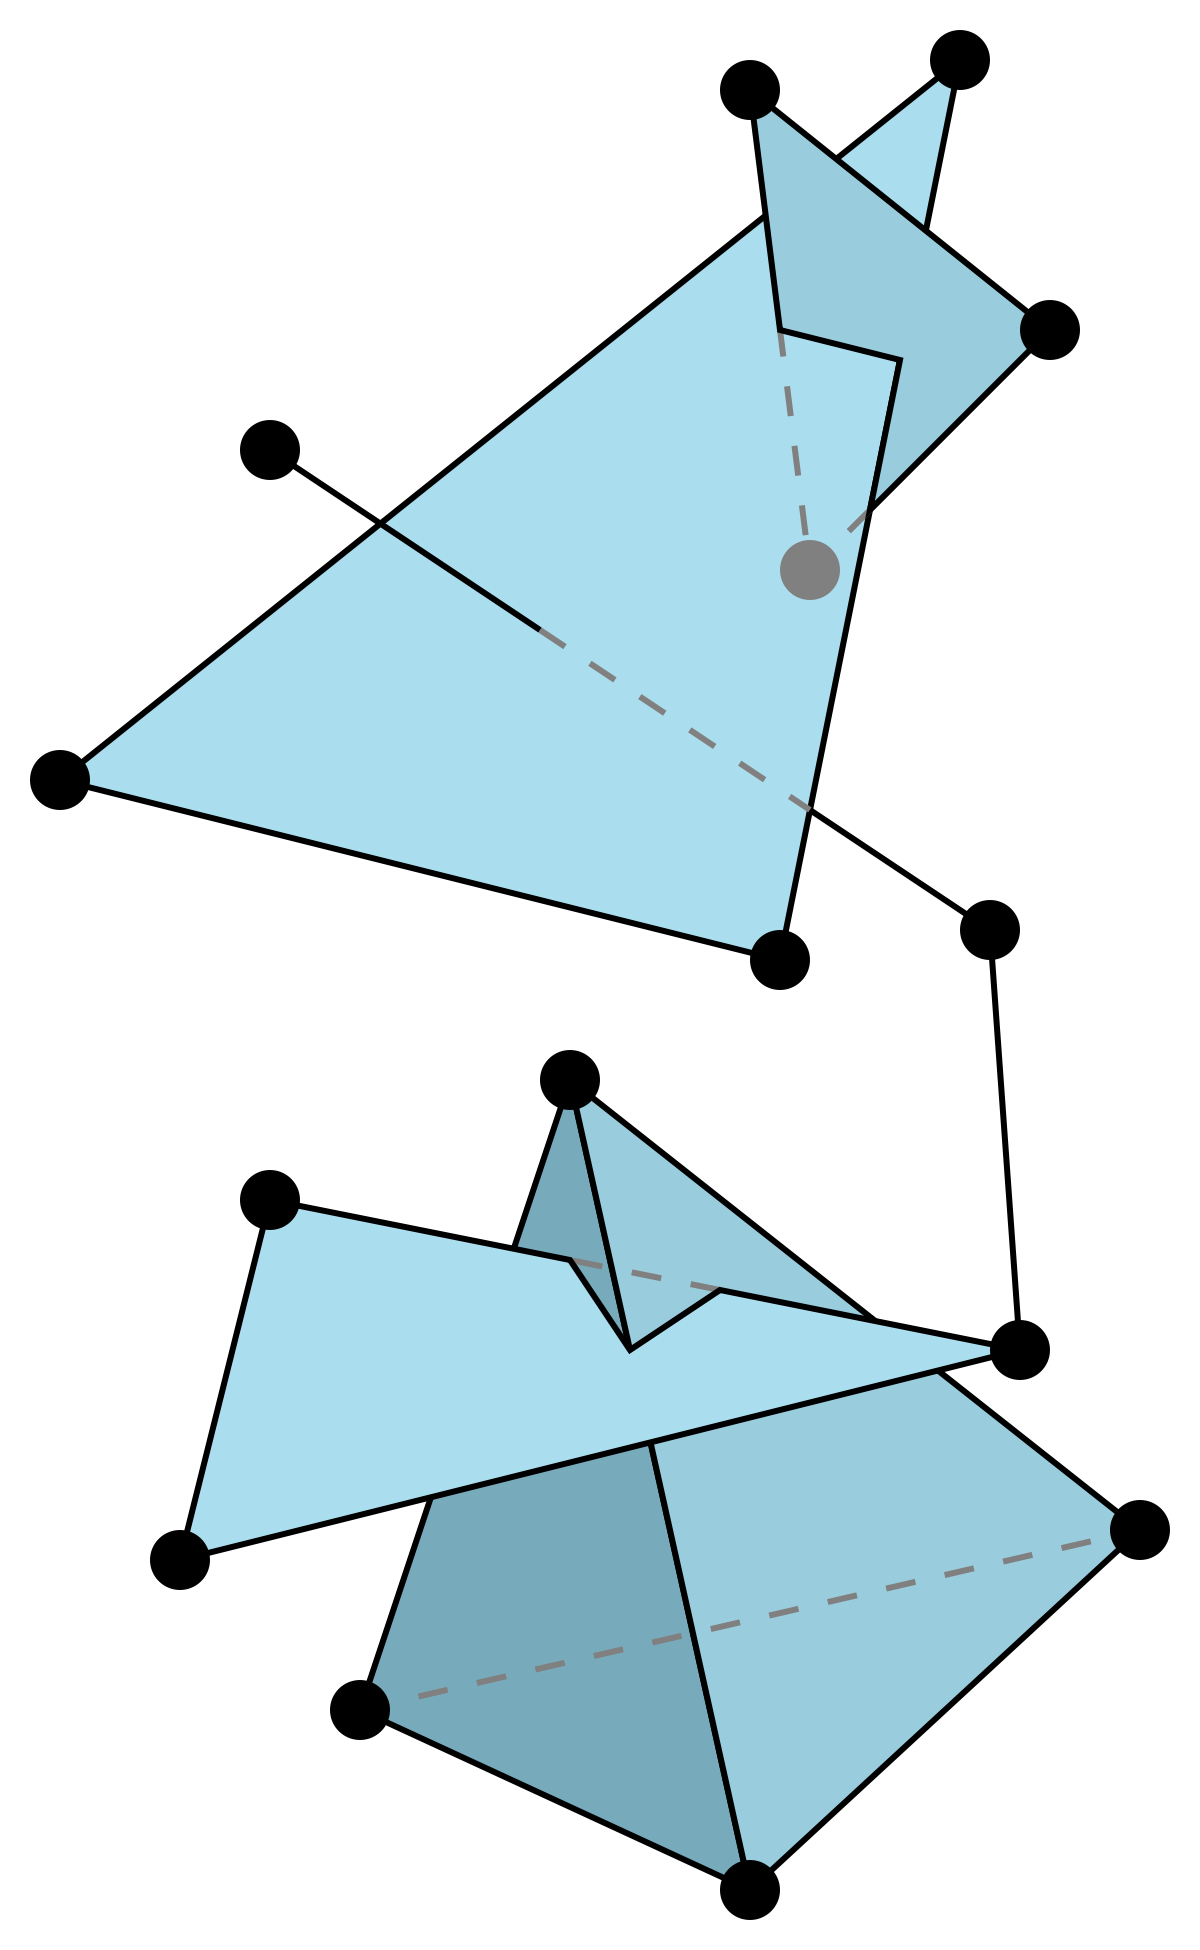
\includegraphics[width=3cm, height=5cm]{sections/1/noncomplex}
        \caption{Set of simplexes which is not a simplicial complex.}
        \label{fig:3}
    \end{figure}

    In fact, we can see in \autoref{fig:3} that the intersection property of simplicial complexes is not satisfied.
\end{document}
